\documentclass{amia}
\usepackage{graphicx}
\usepackage[labelfont=bf]{caption}
\usepackage[superscript,nomove]{cite}
\usepackage{color}
\usepackage{wrapfig}

\begin{document}

\title{Creating RDF data on trauma care organizations from questionnaires}

\author{Joseph R. Utecht, BA$^{1}$,Mathias Brochhausen, PhD$^{1}$, Firstname B. Lastname, Degrees$^{2}$}

\institutes{
    $^1$University of Arkansas for Medical Science, Little Rock, AR, USA; $^2$Institution, City, State, Country (if applicable)\\
}

\maketitle

\noindent{\bf Abstract}

\textit{This abstract should eventually be between 125-150 words long and the paper itself must be between 5 and 10 pages long.}

\section*{Background}
In the United States, injury is the leading cause of death for persons below the age of forty-four and is the fourth leading cause of death overall. The cost of fatal injury and violence in the US was 671 billion dollars in 2013. Trauma systems, which form a single cohesive operating unit that brings together many facets of health care (e.g., injury epidemiology, regional communication centers, prehospital care, hospital-based trauma care, and rehabilitation), have been shown to both decrease mortality and improve quality of care. A recently developed protocol for assessing impact of trauma systems on patient outcome stressed the fact that it is not sufficient to look whether a trauma system exists or not, but that it is crucial to take into consideration trauma system components, such as oversight (lead agency, trauma system plan, etc.), prehospital care (EMS agencies, etc.), definitive care (facility designation, inclusive design, etc.) and rehabilitation. The same is likely to be true for trauma centers, an integral component of trauma systems, that have also been shown to improve patient outcomes without specific reference to system participation. 

The CAFE (Comparative Assessment Framework for Environments of Trauma Care) project (1R01GM111324) aims to address the problem of lack of data about trauma system and trauma center components by allowing users to enter data about their institution (either trauma system or trauma center) and compare it in real-time to other institutions of the same type. Three key requirements of the CAFE project for its infrastructure are 1) the ability provide a semantically-rich vocabulary for trauma systems, trauma centers, and their components and 2) a way data representation that captures the relations between components and allows for different types of relations, 3) user-friendly data entry about components and procedures of trauma systems and trauma centers. The ability to represent semantically-rich data is of utmost importance, since the names of trauma system or trauma center components, e.g. lead agency, trauma medical director, trauma program manager, etc. are experiencing wide-spread while. The problem is that the actual definition of those components and differ considerably from one organization to the other.

In this paper we describe the methodologies used to build the basic CAFE infrastructure, consisting of data entry, data storage, and data retrieval and we will describe the outcome of applying these methodologies. One example for that is reporting. Whom the trauma medical director reports to and whether the trauma program manager reports to the trauma medical director, provided that these two roles exist in an organization, can be completely different from one organization to the other. Representing complex relations and how the existence of those relations can influence the definition of organizational roles, thus is one of the main concerns of the project.



\section*{Methods}
\textcolor{blue}{Explain the basics of the semantic web, hopefully inside of a single paragraph. - Mathias}

The requirements for data representation and information management in the CAFE project include a computer-parsable, semantically-rich vocabulary and the ability to store and represent complex relationships between the components of trauma systems and trauma centers. Due to these requirement we decided to use semantic web technologies to store, manage and extract the data we aim to curate. In the following we briefly describe the semantic web standards we use to fulfill the requirements outline above.

The Web Ontology Language (OWL2) allows computer-parsable and semantically-rich representation of individuals and types in a domain of interest. The latter can be defined axiomatically. 

An adequate way to represent complex data with multiple relations and definition based on those definition Semantic Web Technologies seemed to us to be the most appropriate technologies. The Resource Description Framework (RDF), the basic standard of the Semantic Web allows the representation of entities and multiple relations this entities have to other entities. For our purpose we also plan to use an ontology coded in the Web Ontology Language (OWL2). Ontologies are formal representation of the entities and the relations in a domain of discourse. They enable providing axiomatic definitions of types of entities, e.g. trauma system, trauma medical director, and lead agency. Our strategy is to store the information acquired through the questionnaires as RDF data. Hence, we also need a query language to allow us to run queries over our RDF data. The standard query language for this purpose is SPARQL.

\begin{wrapfigure}{r}{0.7\textwidth}
  \begin{center}
    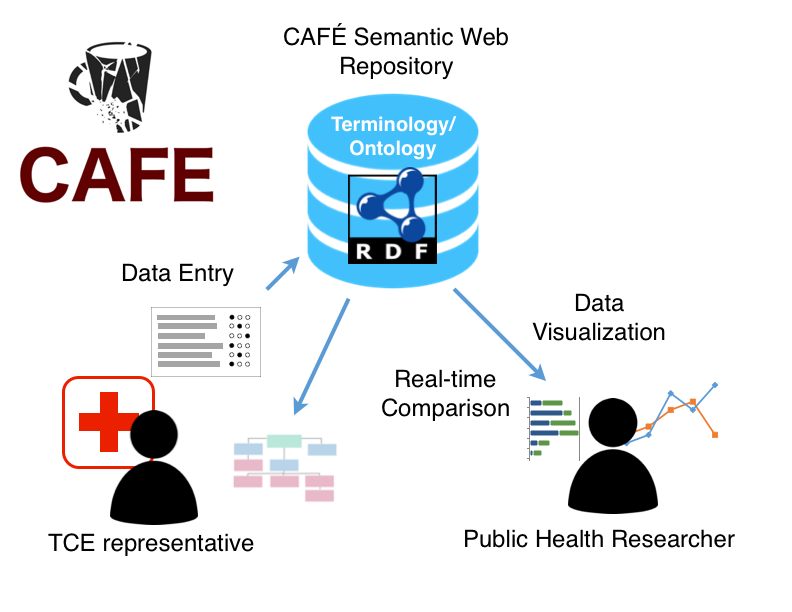
\includegraphics[width=0.68\textwidth]{pics/cafe_figure.png}
  \end{center}
  \caption{CAFE Project Process.}
  \label{cafe_figure}
\end{wrapfigure}

\textcolor{blue}{Maybe this goes after the description of the general outline of the project. Also, we will need citations for all of the standards mentioned}

\textcolor{red}{What level of familiarity with the semantic web should we assume?}
\textcolor{red}{JB: The AMIA 2016 proceedings are over 2000 pages long, and have only four papers that mention "semantic web." So it's not all that common. But a paragraph should be enough.}

The application of this process is a focus of the CAFE project (Figure ~\ref{cafe_figure}).
To those means we have built tools for this purpose.
The main tool is the CAFE questionnaire, which is a web questionnaire to be filled out by trauma center administrators.
The tool records all answers directly into RDF, and will eventually allow users to perform comparisons to other organizations through semantically enriched queries.
It will also build a semantic representation of their organization which will be made available to public health researchers.

\begin{figure}[h]
  \centering
  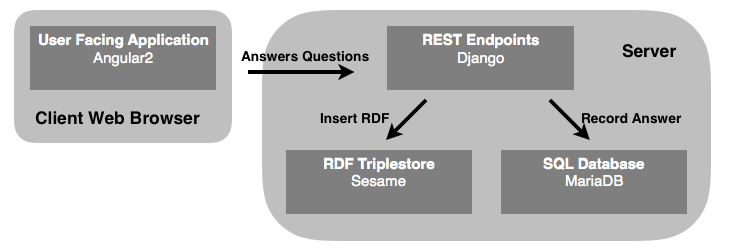
\includegraphics[width=1\textwidth]{pics/cafe_process.png}
  \caption{Components of the CAFE Application.}
  \label{cafe_process}
\end{figure}

\pagebreak

\section*{Results}
\begin{wrapfigure}{r}{0.5\textwidth}
  \begin{center}
    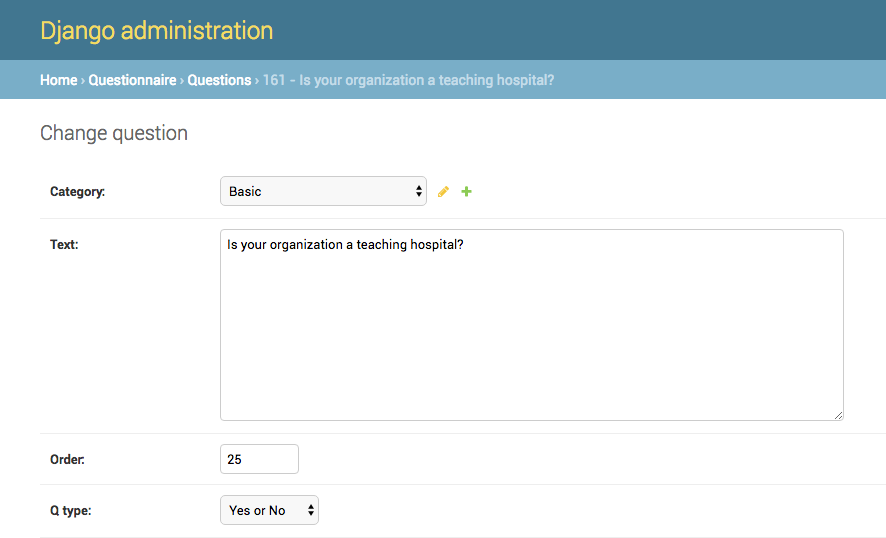
\includegraphics[width=0.48\textwidth]{pics/161_question_admin.png}
  \end{center}
  \caption{Creating a Question in the Administrator Interface.}
  \label{161_question_admin}
  \vspace{5mm}  
   \begin{center}
    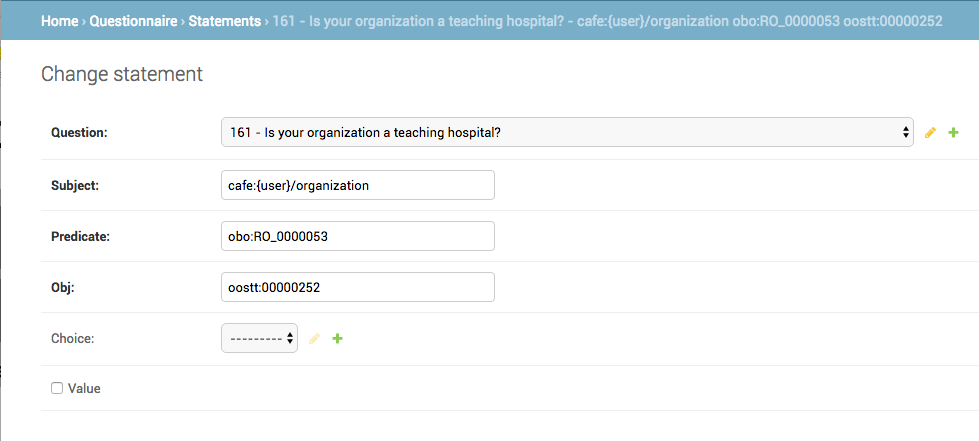
\includegraphics[width=0.48\textwidth]{pics/161_statement_admin.png}
  \end{center}
  \caption{Adding RDF Statements to a Question in the Administrator Interface.}
  \label{161_statement_admin}
\end{wrapfigure}

\textcolor{blue}{What do we actually want to say in the results section?}

\textcolor{red}{Maybe mention semantic survey here, or would that be better for future work?}

The CAFE web application is a custom made site, built using Angular2 and Django, the source of which is available on Github (https://github.com/cafe-trauma/).
The questionnaire currently consists of just over 150 questions with various types of possible answers.
New questions are added to the site through an administrator interface by non-developers (Figure ~\ref{161_question_admin}).
Currently supported are yes/no, number field, check-box selection, and drop downs.
The answers to these questions have RDF representations also entered into the site through the administrator interface by a non-developer. (Figure ~\ref{161_statement_admin})
The RDF representations are created one triple at a time using the standard subject, predicate, and object format.
These can range from a single RDF triple (Figure ~\ref{simple_rdf}) to a complex set of triples (Figure ~\ref{complex_rdf}).
\textcolor{red}{Should we explain what the RDF in these two figures is showing?}
The two previous figures mentioned were generated by the tool to assist the maintainer in visualizing the triples that they are creating for each question.
The questions and RDF statements to be inserted are stored in a relational database and accessed by the Angular2 front-end through a series of REST endpoints handled by Django on the server-side.
When a user answers a question in the positive, either yes on a yes/no or any selection on the other question types, the configured RDF for that question will be inserted into a triplestore on the server.
These triples will be inserted with a context tying them to this user and question, allowed them to be removed if the user changes an answer or queried individually if needed.
This RDF can also be generated later at anytime as the tool also records all answers to the questionnaire in the same relational database which holds the questions and potential triples.
From the users point of view the questionnaire does not differ in any way from a more typical questionnaire backed by a relational database.

\begin{figure}[b]
  \centering
  \begin{minipage}[b]{0.32\textwidth}
    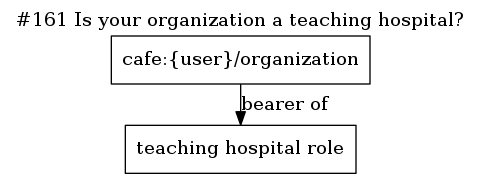
\includegraphics[width=\textwidth]{pics/161.png}
    \caption{Single RDF Triple.}
    \label{simple_rdf}
  \end{minipage}
  \hfill
  \begin{minipage}[b]{0.67\textwidth}
    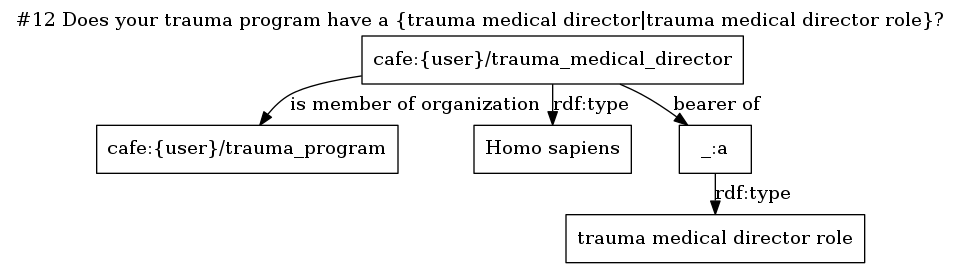
\includegraphics[width=\textwidth]{pics/12.png}
    \caption{More complex RDF example.}
    \label{complex_rdf}
  \end{minipage}
\end{figure}

\textcolor{red}{Also mention ability to share "original data" for the purpose of reproducibility and better transparency in science}

\section*{Discussion}
What we have set forth here is methodology for representing the answers to questionnaires directly into RDF.

\textcolor{red}{Advantages of semantic web, sharability/usability of generated data, question framing}

\section*{Future Work}
Another application we have built using this framework is the DIDEO(?) - evidence of potential drug-drug interaction classification tool.
In this tool trained users will enter properties from reported potential drug-drug interactions through a small number of questions.
These questions will generate RDF in the same way as the CAFE application.
After the questions are answered a logical reasoner is run over the generated RDF which can infer additional properties thus minimizing the number of questions the user will need to fill out.
In this example we are asking the user to answer 10 questions which using this inference can record the same amount of information that it would normally take many more questions to specify.

In both of these example applications the user is presented with a familiar looking survey presentation, but their answers will produce a semantically rich representation of what the questions are asking.  The generated data is immediately ready to be used with any existing RDF data or even translated back into a relational database format with all of the logical inferences intact.

\section*{Parking Lot}
Questionnaires are frequently at the core of biomedical research, such as clinical trials. In these a subject or researcher will enter data.
The questions on this questionnaire will attempt to ascertain whatever information would be useful in the current research.
There is much writing and research into how to properly word questions and design questionnaires so that the research can more accurately capture the information they desire.
However, there is less to be said about how to represent the answers to said questions.
A commonly used method is to simply record the exact answers to the question.
For example on a questionnaire related to smoking, if the question was worded "How many cigarettes a day do you smoke?", and the subject answered twelve the number '12' would be recorded in whatever form was being used to track answers.
This shouldn't cause a problem for the original researcher as they know that the answer '12' is to the question related to number of cigarettes smoked.
A problem arises when this information needs to be compared to another source of data, either a later wording of the question or a separate study.


Imagine a second study where they were only interested in studying "heavy smokers".
The questionnaire in this study asked a question to find heavy smokers "Is the subject a heavy smoker?", and this would have been represented with Yes/No or True/False.
Now later when comparing the data from these two studies in an attempt to make a larger research cohort you come to the problem of how to compare the answer of 'Yes' to the number '12'.
There is the obvious problem of what the definition of a "heavy smoker" in the second question is, but assuming that this is a well known number say greater than 10 cigarettes a day, it will still require human intervention to map the data in to form or the other.
You cannot accurately map the "Yes" of heavy smoker into a specific number of cigarettes a day.
This means the data can only be mapped to the less specific form of heavy smoker yes/no.
In the new dataset we would lose the information of exactly how many cigarettes the subject smoked per day.
This does not even address the issue of what happens if the definition of "heavy smoker" changes over time, when comparing two studies using the same question.

We propose a different way of recording the answers to the questions, which more accurately represents what the question is asking.

\makeatletter
\renewcommand{\@biblabel}[1]{\hfill #1.}
\makeatother

\bibliographystyle{unsrt}
\begin{thebibliography}{1}
\setlength\itemsep{-0.1em}

\bibitem{ref1}
Pryor TA, Gardner RM, Clayton RD, Warner HR. The HELP system. J Med Sys. 1983;7:87-101.
\bibitem{ref2}
Gardner RM, Golubjatnikov OK, Laub RM, Jacobson JT, Evans RS. Computer-critiqued blood ordering using the HELP system. Comput Biomed Res 1990;23:514-28.

\end{thebibliography}

\end{document}
